\section{Representation Analysis: Comparison, Localisation, and Control}
\label{sec:representation}

Following Section~\ref{sec:intermediate-computation}'s emphasis on understanding representations at a broader level, this section considers three successive questions about model representations. Model diffing (Section~\ref{sec:model-diffing}) asks what differs between two models' representations. Knowledge localisation (Section~\ref{sec:knowledge-localization}) asks where a particular piece of information or behaviour is most causally relevant. Representation engineering and steering (Section~\ref{subsec:steering}) asks whether mechanistic understanding of model representations can be used to change model behaviour.

These methods are also closely connected to neighbouring sections. Diffing two checkpoints of the same model can be viewed as a specific instance of the longitudinal analysis discussed in Section~\ref{sec:ld-longitudinal}. Knowledge localisation operates at a coarser level of analysis than the feature-extraction methods in Section~\ref{sec:sae}, but pursues a stricter causal objective by identifying the components at which particular behaviours can be most effectively intervened upon. Finally, representation steering causally tests mechanistic findings by examining whether intervening on an identified representation produces the predicted behavioural change.

\subsection{Model Diffing}
\label{sec:model-diffing}

Many concerning behaviours, such as reward hacking or sycophancy, arise during fine-tuning (\citeestalp{sharma_towards_2025}; \citeemalp{macdiarmid_natural_2025}). This phenomenon makes it important to monitor features and circuits introduced or amplified during this process to prevent unsafe models from being deployed. Model diffing~\citeem{anthropic2024modeldiffing} can surface some of these features. 

\begin{definitionbox}[Model Diffing]
For two models, \emph{model diffing} seeks to identify differences in features or circuits between them. These differences may consist of features or circuits that are exclusive to one model, or of differences in how shared features or circuits are used.
\end{definitionbox}

\paragraph{Representation Alignment and Convergent Learning.} An earlier line of work compared internal representations across models using correlation- and mutual information-based measures~\citeem{pmlr-v44-li15convergent}, canonical-correlation methods such as SVCCA and PWCCA~\citeest{raghu_svcca_2017, morcos2018insightsrepresentationalsimilarityneural}, and kernel-based alignment metrics such as CKA~\citeest{kornblith2019similarityneuralnetworkrepresentations}. Related approaches examine whether the representations of one model can be expressed as linear combinations of representations in another~\citeest{wang_towards_2018}. This literature primarily concerns \emph{convergent learning}: whether independently trained models with different random initialisations learn similar representations up to permutation, rotation, or other linear transformations. More recent work has extended these techniques to study representational convergence across modalities~\citeest{huh2024platonicrepresentationhypothesis, groger2026revisiting}, as discussed in Section~\ref{subsec:universality}.
In contrast to model diffing as defined here, these methods typically focus on representational similarity rather than on identifying concrete features or circuits that are \emph{introduced, amplified, or repurposed} by a specific training intervention.

\paragraph{Applications.} Model diffing has been applied to assess the effect of fine-tuning~(\citeemalp{minder_overcoming_2025, lindsey2024sparsecrosscoders, aranguri2025modeldiff}; \citeestalp{wang2026persona}) and distillation~\citeem{baek_towards_2025}, to track differences between model architectures~(\citeestalp{thasarathan_universal_2025}; \citeemalp{jiralerspong_cross-architecture_2025}), to study the evolution of concepts during pretraining~\citeest{bayazit-etal-2026-crosscoding, ge2026evolution}, and to identify vision-specific features introduced during vision-language training, enabling targeted removal or steering~\citeem{batra2026multimodalmodeldiffingfeature}.


\paragraph{Dictionary Learning Methods.} Dictionary learning is an intuitive approach to implement model diffing. It can highlight unexpected, newly introduced features of concern. When diffing models of the same architecture, such as a base versus instruction-fine-tuned model or a series of model checkpoints along pretraining, dictionary learning methods like sparse autoencoders (SAEs) and transcoders can be trained on the difference in token activations~(\citeemalp{dumas_what_2025, sawmya2025birth}; \citeestalp{inaba2025howllmslearn}). This difference can capture features introduced by fine-tuning or by different pretraining stages. A simple baseline technique is to train an SAE on the base model alone and use it as a fixed feature basis for comparison. Methods like SAE-Track maintain continuity through recurrent initialisation, training each checkpoint's SAE from its predecessor's so latents remain matched across the run~\citeem{xu2024saetrack}. The differences in activations between two models are then measured on a shared evaluation prompt set~\citeest{wang2026persona}. By causally intervening with latents that activate more strongly in the fine-tuned model, it is possible to identify features responsible for misaligned behaviour~\citeest{wang2026persona}.

One challenge for model-diffing approaches is attributing features in a fine-tuned model's representations to the fine-tuning itself. To address this, an SAE trained on a base model can be fine-tuned stage-wise~\citeem{bricken2024stagewise}: first on the base model with fine-tuning data, then on the fine-tuned model with base data, and finally on the fine-tuned model with fine-tuning data. Only features exclusive to the last setting are likely to have been introduced via fine-tuning.

SAEs are applicable when inputs from different models have the same dimension. When diffing two models with different architectures, for example, to track dispositions across model generations or sizes, this might not hold. In this case, crosscoders offer an alternative (Figure~\ref{fig:diffing}). Crosscoders can define model-specific encoders with arbitrarily different input dimensions that project activations from different models into one or more shared representational spaces. Although the main advantage of crosscoders over SAEs is cross-architecture comparison~(\citeestalp{thasarathan_universal_2025}; \citeemalp{jiralerspong_cross-architecture_2025}), some prior work has also applied them to base and fine-tuned models~\citeem{lindsey2024sparsecrosscoders, bricken2024stagewise, minder_overcoming_2025} and across pretraining checkpoints~\citeest{ge2026evolution, bayazit-etal-2026-crosscoding}.

A related approach is to model differences in how representations are \emph{transformed}, rather than comparing the representations themselves. \citetem{hu2026transcoderadaptersreasoningmodeldiffing} used transcoders to learn a function that approximates the difference in MLP computation between a base model and its fine-tuned variant. Specifically, adapters are trained so that a base MLP augmented with a learned correction term reproduces the fine-tuned MLP's behaviour within the full model. Unlike the above methods, which operate on activation differences, this method learns a transformation that approximates how fine-tuning modifies the model's MLP computation. 

A shared concern across dictionary-learning-based model-diffing methods is the faithfulness of the sparse decomposition (see Section~\ref{subsubsec: sae limitation}). Extracted features may not faithfully reflect the underlying representations or their causal roles, potentially leading to false-positive findings about differences between models. For example, identifying an SAE feature associated with ``confessing previous faults'' in a fine-tuned model but not in the original does not establish that the fine-tuned model causally uses this feature. Nor does its apparent absence from the original model imply that the model lacks representations that could steer it towards such behaviour.

\begin{warningbox}[False Positives in Model Diffing]

Dictionary learning methods for model diffing risk falsely identifying model-exclusive features~\citeem{minder_overcoming_2025, jiralerspong_cross-architecture_2025}. This can result from the loss function: for instance, \citetem{minder_overcoming_2025} showed that crosscoders trained with an $L_1$ regularisation on hidden states can falsely identify novel features, which they tried to mitigate with $\sigma_{\text{Batch-TopK}}(\cdot)$. However, even with this improved architecture, false positives may persist. During fine-tuning, the directions representing some features can rotate, and dictionary learning methods currently cannot distinguish between features introduced via fine-tuning and those merely represented differently. Thus, supposedly model-exclusive features should be regarded as hypotheses that need further validation. 
\end{warningbox} 

\paragraph{LLM-Based Approaches.} To differentiate closed-weight models, it is desirable to develop model diffing tools that only rely on API access. To that end, \citetem{kempf2026simplellmbaselinescompetitive} showed that an LLM can generate natural-language hypotheses about behavioural differences between two models by extracting, clustering, and summarising differences across many response pairs from the two models on a shared prompt set. Benchmarked against the SAE-based baseline, the LLM-based method matches it on many dimensions while surfacing more abstract, behaviour-level differences.

\begin{figure}[tb]
  \centering
  \centering
    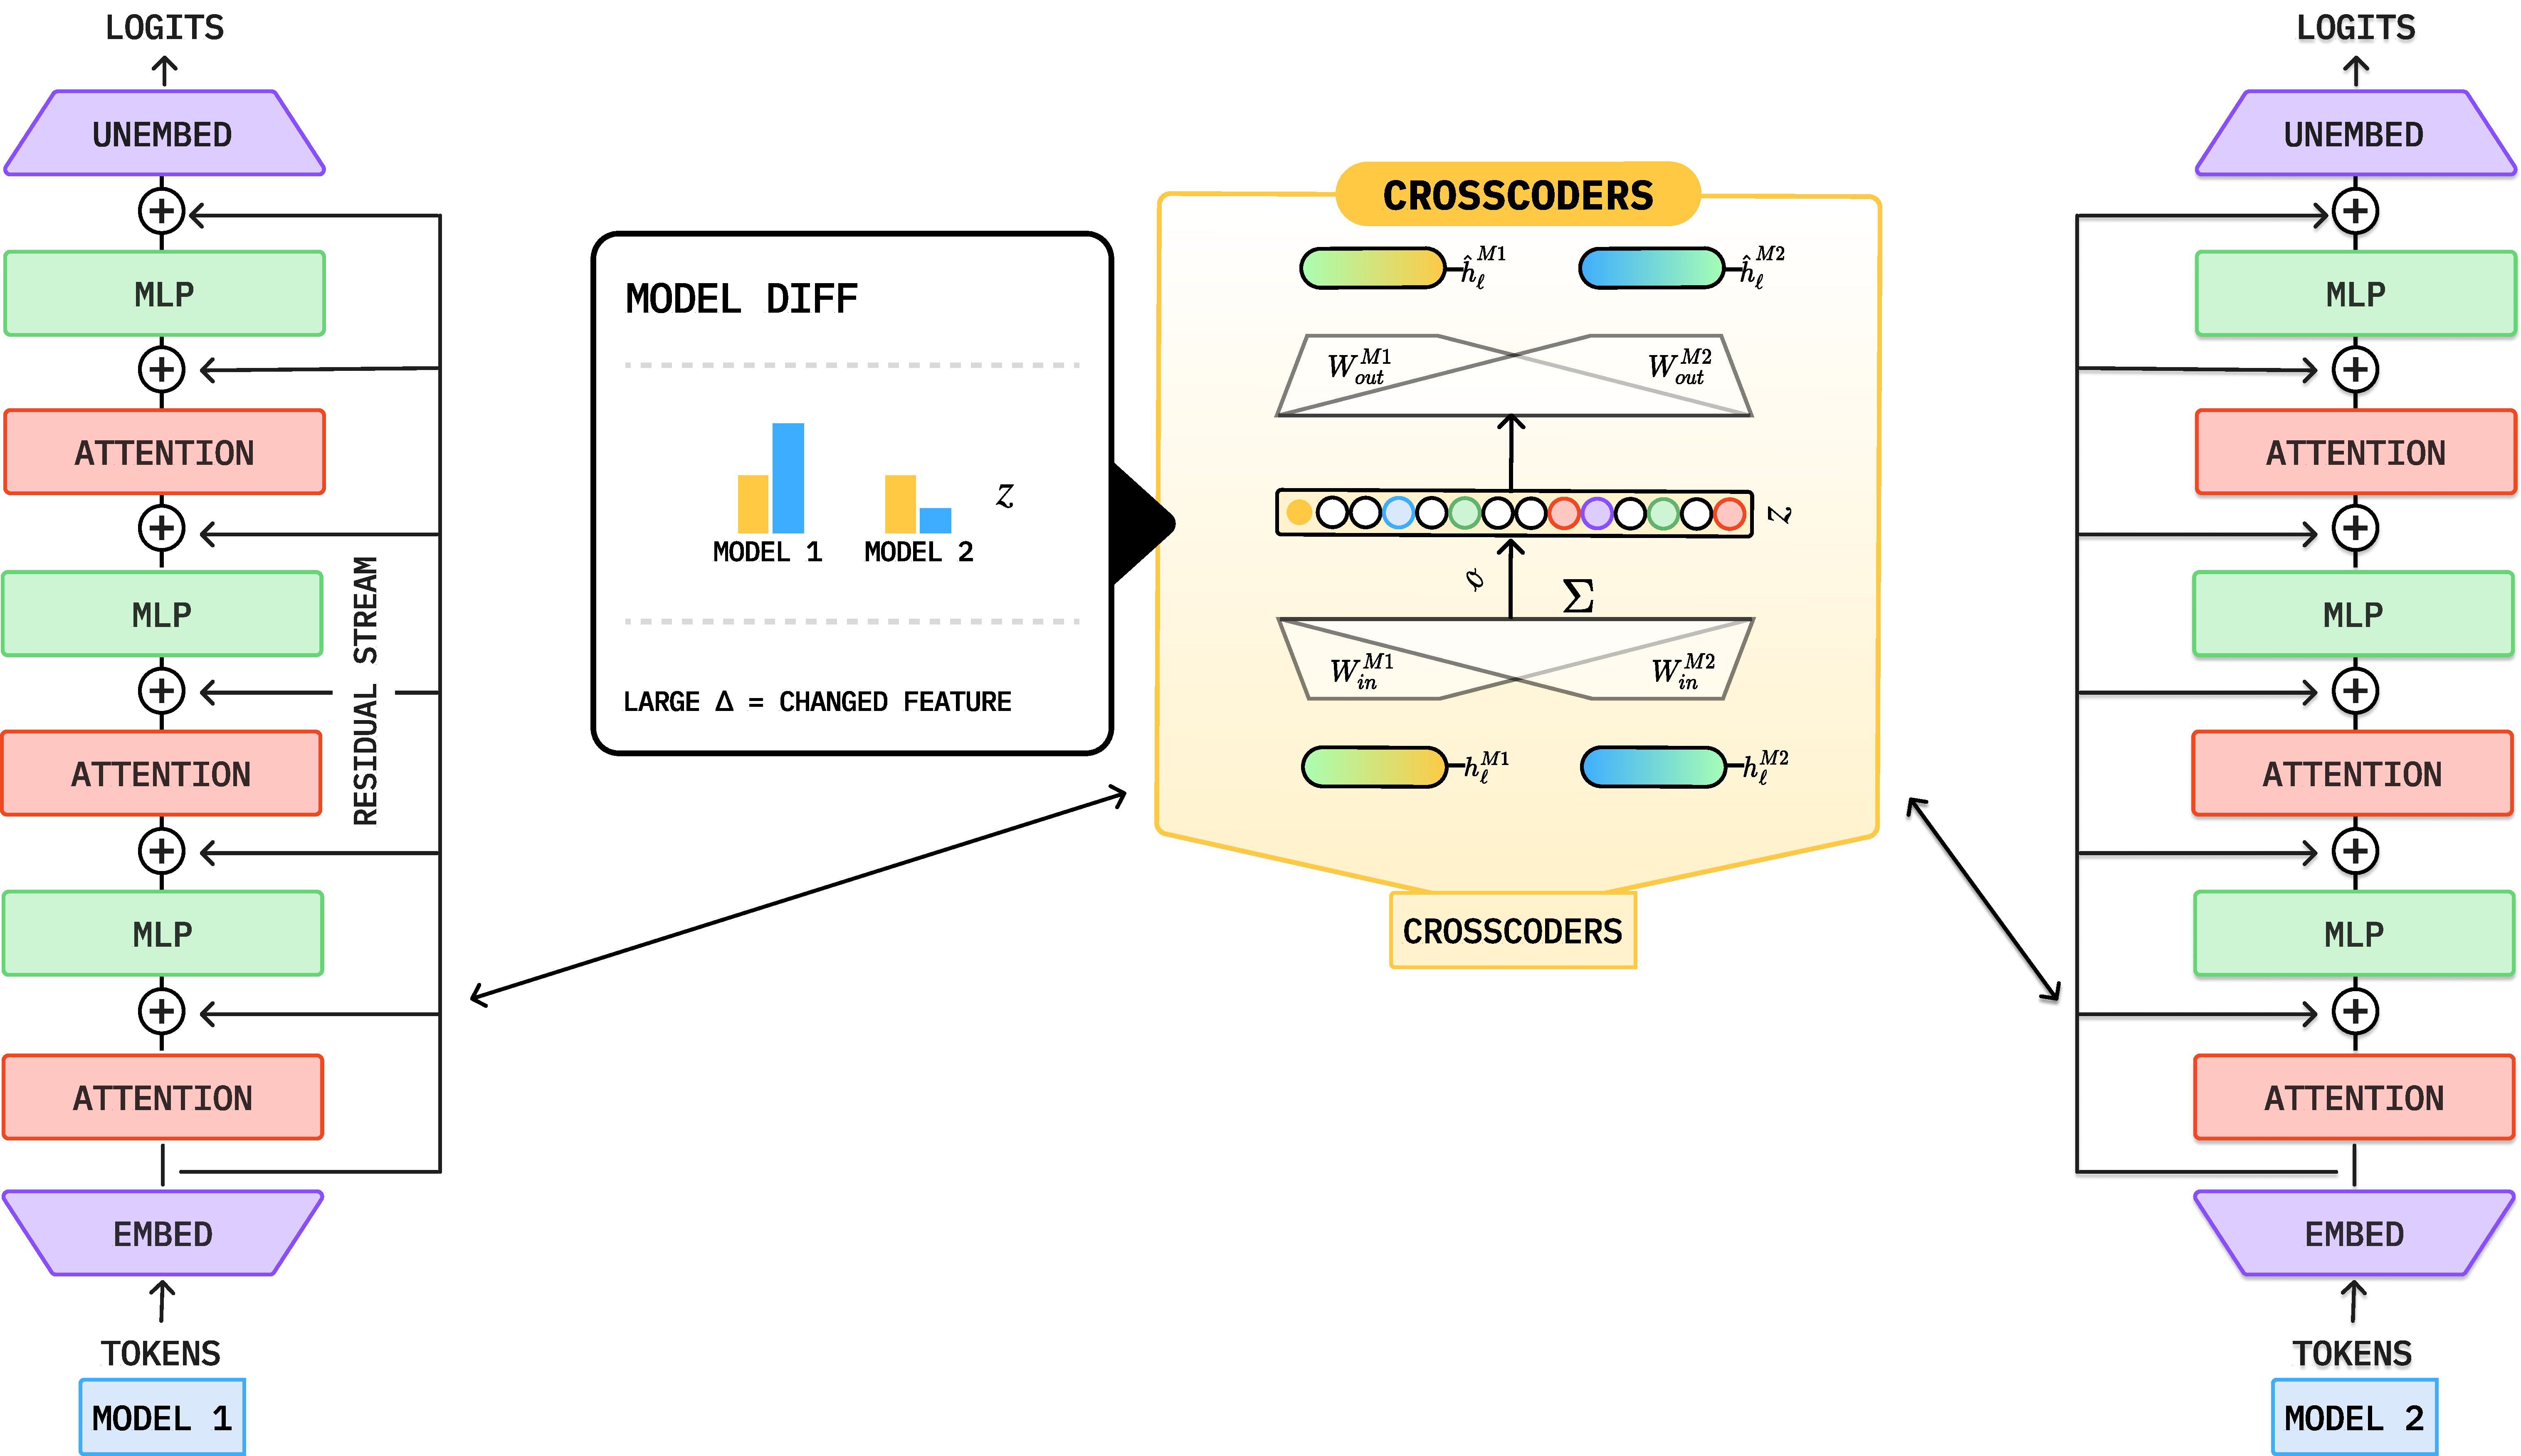
\includegraphics[width=\linewidth]{figs/11_ModelDiffing.pdf}
    \caption{\textbf{Model diffing via crosscoders.} Model diffing identifies features that emerge or remain invariant across model iterations or architectures. A large delta ($\Delta$) in feature activation between two models highlights a changed feature, providing an insight into how fine-tuning or architectural changes alter internal representations.}
    \label{fig:diffing}
\end{figure}

\subsection{Knowledge Localisation}
\label{sec:knowledge-localization}




Knowledge localisation methods aim to identify the layers, components, or subspaces whose activations causally relate to a particular capability or behaviour. This practice draws on the hypothesis that certain information concentrates in specific model locations. For example, \citetest{geva-etal-2021-transformer} proposed that feed-forward layers can mechanistically act as key--value memories; \citetest{dai-etal-2022-knowledge} found that factual knowledge associations are stored in them; and \citetest{sharma2024the} discovered that the information of these associations mainly flows through the subspace spanned by the top singular directions of late-layer MLPs' weight matrices. These analyses laid the groundwork for knowledge localisation and motivated corresponding techniques~\citeest{meng2023locatingeditingfactualassociations}.

Localisation can identify the components where a behaviour or piece of knowledge is most decodable or most causally influential. It has been a standard first step for many intervention-based analyses, such as steering vectors (Section~\ref{subsec:steering}), probes (Section~\ref{subsec:probing}), and knowledge editing (Section~\ref{subsec:knowedit}). However, localisation alone does not reveal how the relevant information is computed or represented. In transformers, which are usually overparameterised, information can be redundantly represented and processed across many model components and activation subspaces depending on the input. A component with a strong causal effect may capture only a small part of the mechanism. As a result, localisation is a useful starting point for mechanistic understanding, but not a self-contained analysis.

For steering vectors and probes, localisation usually means finding the most effective layer or token position to steer or probe model activations. For example, \citetest{arditi2024refusallanguagemodelsmediated} searched over layers and post-instruction token positions to identify the most performant difference-in-means vector for steering the model towards or away from refusal behaviour. Similarly, \citetem{macdiarmid2024sleeperagentprobes} studied the sleeper-agent behaviour~\citeem{hubinger2024sleeperagentstrainingdeceptive} by comparing and probing activations across layers for triggered and non-triggered inputs. In knowledge editing, localisation often means identifying the MLP blocks that stores the knowledge of interest to modify. A classical technique is causal tracing~\citeest{meng2023locatingeditingfactualassociations}, which identifies components that causally affect specific factual association retrieval by observing how model outputs change after activation intervention, and is used in editing methods like ROME~\citeest{meng2023locatingeditingfactualassociations}, MEMIT~\citeest{meng2023masseditingmemorytransformer}, and AlphaEdit~\citeest{alphaedit}. In sum, this localisation practice, along with intervention methods, has become an established pipeline for answering where and how the model encodes behaviour- or knowledge-related information. However, identifying a model module, layer, or activation subspace does not explain the internal mechanisms underlying the behaviour, which can only be understood through finer-grained analyses such as circuit discovery.

\subsection{Representation Engineering and Steering}
\label{subsec:steering}




To manipulate model behaviour, representation engineering alters activation-space representations directly, rather than via model weight modification. \emph{Activation steering} generally refers to methods that target intermediate activations (usually the residual stream) by adding certain vectors that shift model outputs during inference. This differs from localisation methods, which determine where information or behaviour is represented, as steering techniques aim to identify a specific, manipulable vector that \emph{changes} model behaviour. Because they require no weight updates or retraining, these interventions are lightweight approaches for controlling behaviour.

\begin{definitionbox}[Steering Vector (Figure~\ref{fig:steering_vectors})]
A \emph{steering vector} $v_{\text{steer}} \in \mathbb{R}^{d}$ is an activation-space direction which, when scaled ($\alpha v_{\text{steer}}$) and added to an intermediate activation, shifts model outputs towards a targeted behaviour. For instance, one steering direction can use the weight vector of a trained linear probe. Another popular method is \emph{difference-in-means}, which obtains the steering vector by taking the difference between activations associated with two behaviours~\citeest{panickssery2024steeringllama2contrastive}:
\[
v_{\text{steer}} =
\mathbb{E}[h_\ell \mid \text{preferred}]
-
\mathbb{E}[h_\ell \mid \text{unpreferred}].
\]
During inference, the intervention takes the form
\[
\tilde{h}_\ell = h_\ell + \alpha v_{\text{steer}},
\]
where $\alpha$ controls the intervention strength.
\end{definitionbox}

While these approaches appear simple, they reliably change model behaviours such as refusal, helpfulness, and stylistic tendencies~\citeest{panickssery2024steeringllama2contrastive,zhao2025steering,arditi2024refusallanguagemodelsmediated}. Thus, steering is useful both as a technique to manipulate behaviour and as a causality test for probes. If intervening along a direction consistently changes a target behaviour, this provides evidence that the corresponding representation causally influences that behaviour. Below we use refusal vectors as a concrete example.

\begin{definitionbox}[Refusal Vector]
\label{def:refusal-vector}



A \emph{refusal vector}~\citeest{arditi2024refusallanguagemodelsmediated} is a steering direction associated with a model's tendency to refuse requests. 
Define $h^t_\ell \in \mathbb{R}^d$ as the residual stream at layer $\ell$ and token position $t$. A simple contrastive construction is
\[
\mathbf{r}_\ell =
\mathbb{E}_{x \sim \mathcal{D}_{\mathrm{refuse}}}
[h^t_\ell(x)]
-
\mathbb{E}_{x \sim \mathcal{D}_{\mathrm{comply}}}
[h^t_\ell(x)],
\]
where $\mathcal{D}_{\mathrm{refuse}}$ contains prompts eliciting refusal behaviour and $\mathcal{D}_{\mathrm{comply}}$ contains matched prompts for which the model should comply.\\

The projection
\[
s^t_\ell = \langle h^t_\ell,\mathbf{r}_\ell\rangle
\]
measures the activation along the refusal direction. When intervening on this direction, one can test if and how refusal behaviour is causally influenced by it. Previous experimental work shows that these interventions can strongly modulate refusal behaviour; however, the construction and interpretation of refusal directions can vary across models and experimental settings~\citeest{arditi2024refusallanguagemodelsmediated}.
\end{definitionbox}

The contrast between \emph{localisation} and \emph{steering} is shown by refusal vectors: measuring $s^t_\ell$ across layers helps locate representations that contain information related to refusal, while intervening along $\mathbf{r}_\ell$ tests how modifying representations modulates behaviour (which provides evidence for causality, but does not necessarily reveal the entire mechanism behind how refusal works).

\paragraph{Nonlinear and Optimisation-Based Steering.}
Beyond linear directions, recent studies have explored more complex ways of manipulating model activations. For example, \citetem{raval2026curveballsteeringrightdirection} projected model activations into a kernel PCA space, steered them linearly there, and projected them back to the original activation space; \citetem{wurgaft2026manifoldsteeringrevealsshared} steered activations along a low-dimensional manifold, motivated by findings that some concepts are better represented as manifolds in the activation space. Separately, optimisation-based methods construct steering directions by directly optimising objectives over intermediate activations, offering an alternative to closed-form constructions. For example, they can be obtained by maximising task performance or by suppressing undesirable outputs under intervention. 
These optimisation-based approaches offer greater flexibility for complex or nonlinear objectives but generally require substantially more computation than closed-form contrastive methods~\citeest{dunefsky2025one, oozeer2025beyond}.

\begin{figure}[tb]
  \centering
    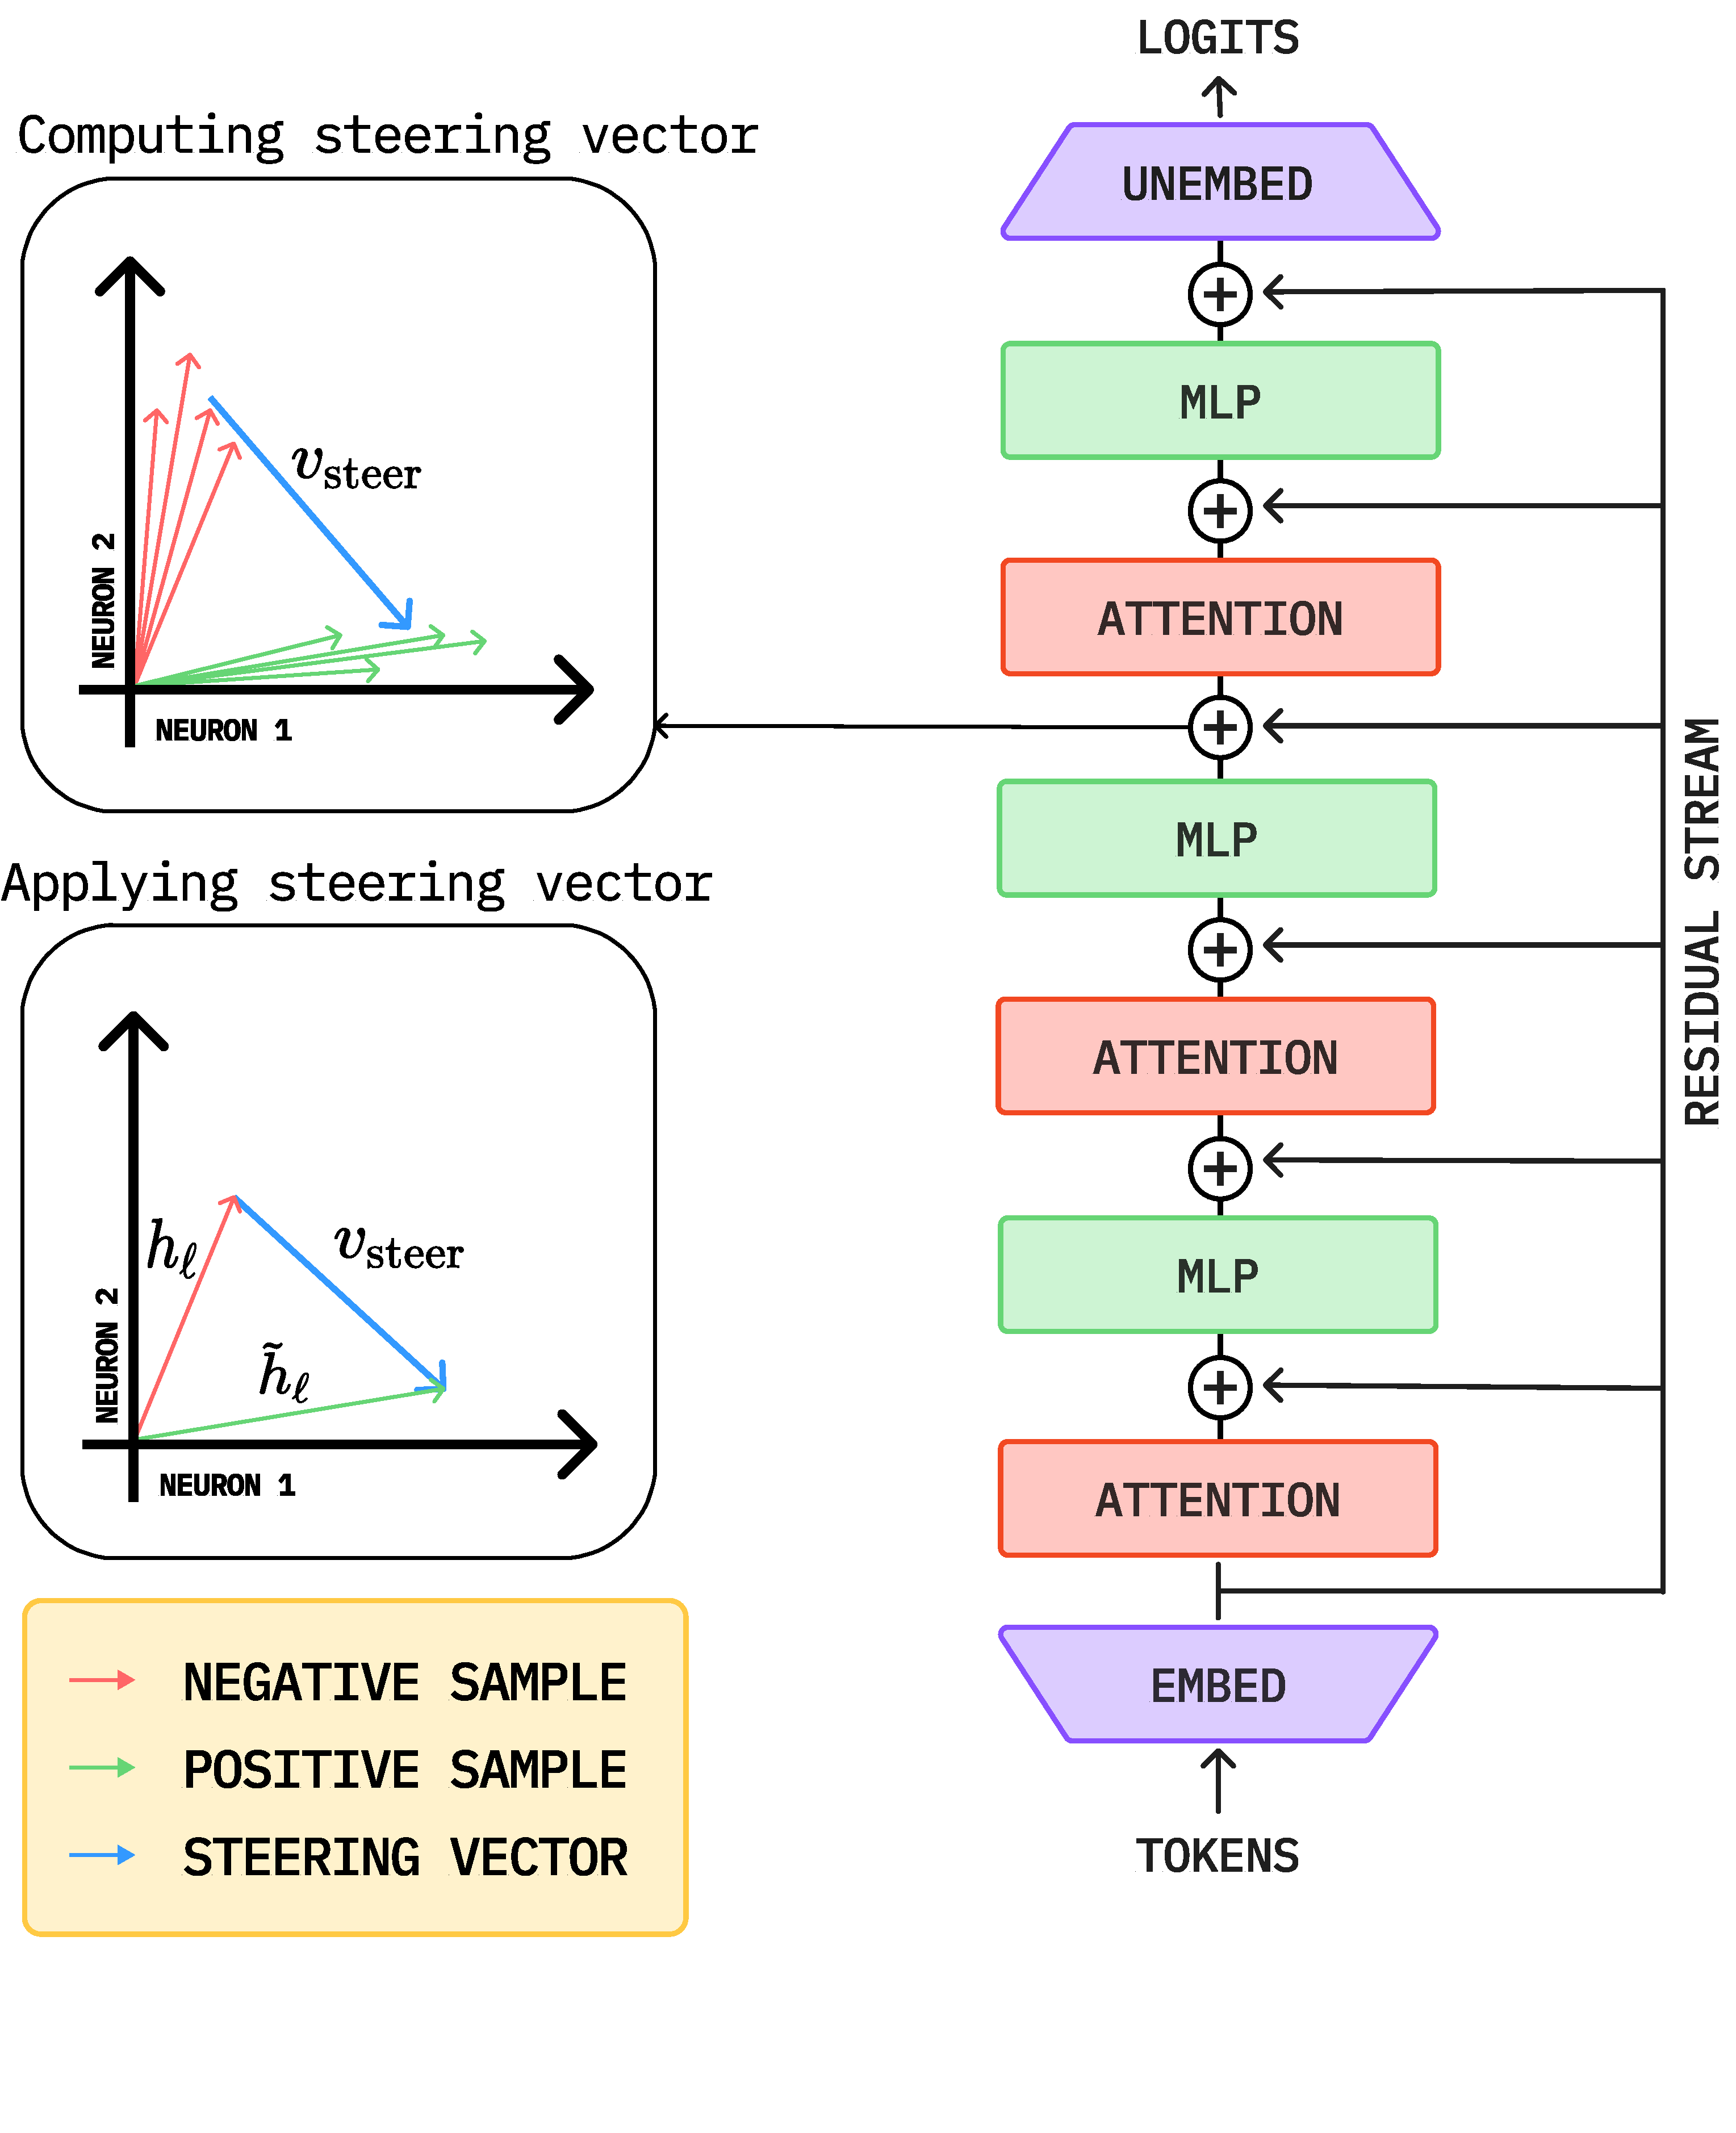
\includegraphics[width=0.5\linewidth]{figs/11_Steering.pdf} 
    \caption{\textbf{Steering Vectors.} A steering vector $v_{\text{steer}}$ can be constructed from the difference between the mean activations of positive and negative contrastive samples at a target layer. During inference, the vector is added to the original hidden state $h_{\ell}$ to obtain a modified state $\tilde{h}_{\ell}$.}
    \label{fig:steering_vectors}
\end{figure}

\paragraph{Steering as a Causal Test for Feature Interpretability.}

Activation steering can causally evaluate representations previously labelled by feature-extraction methods (such as CLTs or SAEs). For instance, a feature may be hypothesised to represent a particular concept. Supporting evidence can be obtained by steering along the identified feature direction and evaluating the resulting change in behaviour. 

These evaluations have been used to compare interpretable direction-identification approaches, including SAE features, difference-in-means directions, and DAS~\citeest{huang-etal-2024-ravel, wu2025axbench}. 
Benchmarks designed to evaluate the causal and behavioural properties of learned representations include RAVEL~\citeest{huang-etal-2024-ravel}, MIB~\citeest{mueller2025mib}, and AxBench~\citeest{wu2025axbench}.

\begin{warningbox}[Limitations: Brittleness and Mechanistic Opacity]
While steering methods effectively control behaviours and support causal testing, they have limitations. Notably, they can be brittle, as a direction identified for one distribution, model, or task may not generalise reliably. Another limitation is that successful behavioural steering does not, by itself, establish mechanistic transparency, because an intervention may simultaneously impact multiple features, interact nonlinearly with existing computations, or exploit unintended pathways that produce the desired behaviour without corresponding to a clean mechanism~\citeest{makelov2024is}. Thus, steering should generally be interpreted as evidence for causal influence, but it should not, by itself, be taken as a mechanistic explanation of the behaviour.
\end{warningbox}


\paragraph{Summary.} Model diffing examines representation differences across models, knowledge localisation pinpoints where information or behaviours are causally localised, and representation engineering analyses how representation manipulation controls behaviour. Steering has two important roles: as a control technique and as a way to causally test how representations affect behaviour (while noting that successful localisation or steering does not, by itself, provide a complete explanation for the mechanism underlying that behaviour). This analysis is extended in Section~\ref{sec:training}, which examines how representations and mechanisms evolve during training.
